\documentclass[10pt,final,a4paper,oneside,onecolumn]{article}

%%==========================================================================
%% Packages
%%==========================================================================
\usepackage[a4paper,left=3.5cm,right=3.5cm,top=3cm,bottom=3cm]{geometry} %% change page layout; remove for IEEE paper format
\usepackage[T1]{fontenc}                        %% output font encoding for international characters (e.g., accented)
\usepackage[cmex10]{amsmath}                    %% math typesetting; consider using the [cmex10] option
\usepackage{amssymb}                            %% special (symbol) fonts for math typesetting
\usepackage{amsthm}                             %% theorem styles
\usepackage{dsfont}                             %% double stroke roman fonts: the real numbers R: $\mathds{R}$
\usepackage{mathrsfs}                           %% formal script fonts: the Laplace transform L: $\mathscr{L}$
\usepackage[pdftex]{graphicx}                   %% graphics control; use dvips for TeXify; use pdftex for PDFTeXify
\usepackage{array}                              %% array functionality (array, tabular)
\usepackage{upgreek}                            %% upright Greek letters; add the prefix 'up', e.g. \upphi
\usepackage{stfloats}                           %% improved handling of floats
\usepackage{multirow}                           %% cells spanning multiple rows in tables
%\usepackage{subfigure}                         %% subfigures and corresponding captions (for use with IEEEconf.cls)
\usepackage{subfig}                             %% subfigures (IEEEtran.cls: set caption=false)
\usepackage{fancyhdr}                           %% page headers and footers
\usepackage[official,left]{eurosym}             %% the euro symbol; command: \euro
\usepackage{appendix}                           %% appendix layout
\usepackage{xspace}                             %% add space after macro depending on context
\usepackage{verbatim}                           %% provides the comment environment
\usepackage[dutch,USenglish]{babel}             %% language support
\usepackage{wrapfig}                            %% wrapping text around figures
\usepackage{longtable}                          %% tables spanning multiple pages
\usepackage{pgfplots}                           %% support for TikZ figures (Matlab/Python)
\pgfplotsset{compat=1.14}						%% Run in backwards compatibility mode
\usepackage[breaklinks=true,hidelinks,          %% implement hyperlinks (dvips yields minor problems with breaklinks;
bookmarksnumbered=true]{hyperref}   %% IEEEtran: set bookmarks=false)
%\usepackage[hyphenbreaks]{breakurl}            %% allow line breaks in URLs (don't use with PDFTeX)
\usepackage[final]{pdfpages}                    %% Include other pdfs
\usepackage[capitalize]{cleveref}				%% Referensing to figures, equations, etc.
\usepackage{siunitx}								%% Appropriate behavior of units
\usepackage[utf8]{inputenc}   				 	%% utf8 support (required for biblatex)
\usepackage{csquotes}							%% Quoted texts are typeset according to rules of main language
\usepackage[style=ieee,doi=false,isbn=false,url=false,date=year,minbibnames=15,maxbibnames=15,backend=biber]{biblatex}
%\renewcommand*{\bibfont}{\footnotesize}		%% Use this for papers
\setlength{\biblabelsep}{\labelsep}
\bibliography{../../bib}

%%==========================================================================
%% Define reference stuff
%%==========================================================================
\crefname{figure}{Figure}{Figures}
\crefname{equation}{}{}

%%==========================================================================
%% Define header/title stuff
%%==========================================================================
\newcommand{\progressreportnumber}{30}
\renewcommand{\author}{Erwin de Gelder}
\renewcommand{\date}{May 6, 2020}
\renewcommand{\title}{Performance assessment of automated vehicles using real-world driving scenarios}

%%==========================================================================
%% Fancy headers and footers
%%==========================================================================
\pagestyle{fancy}                                       %% set page style
\fancyhf{}                                              %% clear all header & footer fields
\fancyhead[L]{Progress report \progressreportnumber}    %% define headers (LE: left field/even pages, etc.)
\fancyhead[R]{\author, \date}                           %% similar
\fancyfoot[C]{\thepage}                                 %% define footer

\begin{document}
	
\begin{center}
	\begin{tabular}{c}
		\title \\ \\
		\textbf{\huge Progress report \progressreportnumber} \\ \\
		\author \\ 
		\date
	\end{tabular}
\end{center}

\section{Previous meeting minutes}

\begin{itemize}
	\item We discussed my idea for the generation of test cases. Jan-Pieter mentioned that I should not forget the static environment.
	\item The focus of the coming period is on the ``scenario risk quantification'' and the ``test case generation''.
\end{itemize}



\section{Summary of work}

\begin{itemize}
	\item In the conference paper that we wrote on the ``scenario risk estimation'', we analyzed the likelihood of a collision within a certain scenario given an automated driving system (ADS). Here, it was assumed that the human did not intervene. As such, we did not consider the \emph{controllability}\footnote{Not to be confused with the notion of \emph{controllability} in system theory.} that ISO~26262 defines as the likelihood that,
	when subject to a hazardous situation, the vehicle driver avoids
	an accident. 
	
	A logical next step in our work would be to consider a driver that might intervene in order to avoid an accident. My idea is very simple: include a model of the driver in the simulations of the test cases and see whether the driver can avoid the accident in case the ADS fails to do so, see \cref{fig:model}. Next, by running many simulations varying the scenario parameters according to the distributions of the parameters estimated using real-world driving data, the \emph{controllability} could be estimated. Although the idea sounds very simple, I have not found any literature attempting to estimating the ``controllability'' in this manner. 
	
	I performed a simple case study in which I analyzed the \emph{controllability} in case a vehicle in front brakes. The scenario was parameterized with three parameters: the initial speed, the total speed decrease during the braking activity, and the average braking deceleration. Based on the data set described in \autocite{paardekooper2019dataset6000km}, I estimated the multivariate distribution of these parameters. I based the driver model on the Intelligent Driver Model (IDM) \autocite{treiber2000congested}. The difference to IDM is that I included a response delay of \SI{0.5}{\second} to account for the response time of the driver and I limited the maximum deceleration to \SI{3}{\meter\per\second\squared}.
	
	The result of the analysis is shown in \cref{fig:result}. It shows the likelihood that a collision occurs if a vehicle in front is braking while driving at a certain speed and at a certain time headway. The \emph{controllability} is the complement of the likelihood that a collision occurs.
	
	\begin{figure}
		\centering
		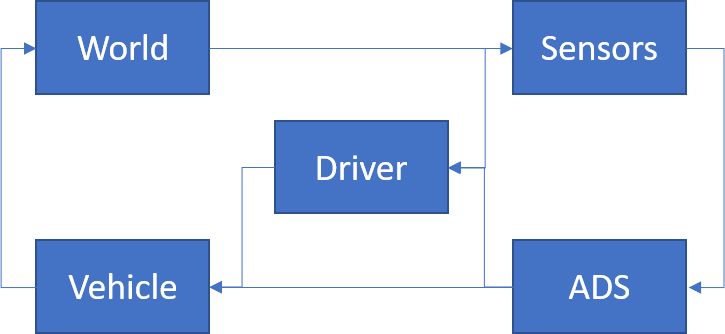
\includegraphics[width=.5\linewidth]{model.png}
		\caption{Simplified scheme of the simulation that includes a driver model.}
		\label{fig:model}
	\end{figure}
	
	\begin{figure}
		\centering
		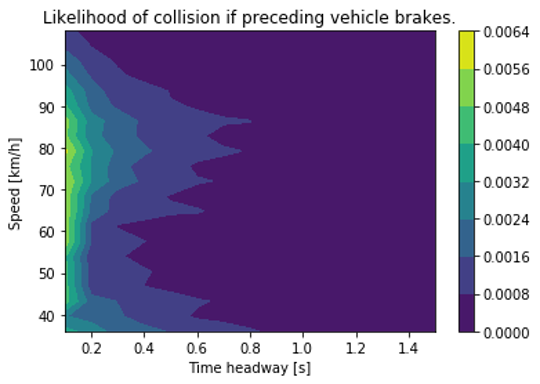
\includegraphics[width=.5\linewidth]{riskresult.png}
		\caption{Estimated likelihood of a collision in case a vehicle in front brakes.}
		\label{fig:result}
	\end{figure}


	\item I continued the work on the test case generation. I completed an example in which I can generate many cut-in scenarios. However, while doing so, I have two concerns:
	\begin{itemize}
		\item I did many assumptions on the dependence/independence of certain parameters. With cross validation, I can check whether certain assumptions make sense, but there are simply too many possibilities to check them all. This makes it hard to come up with a general recipe for generating test cases. 
		\item With the current method, the number of parameters for each test case is not fixed. For example, with the cut-in scenario, the lateral activity of the vehicle that performs the cut in is fixed (a lane change), but in the longitudinal direction, the activities are not fixed. So the vehicle might only cruise or the vehicle first decelerates and then starts to cruise, etc. Each activity introduces new parameters. Potentially, we may also want to vary the number of vehicles and each vehicle also introduces new parameters. Because the number of parameters is not fixed, techniques like Principle Component Analysis (PCA) are not applicable. 
		\item For each test case, we can compute a likelihood based on the parameters. This likelihood is needed if we want to apply techniques such as Markov chain Monte Carlo (this actually only requires a likelihood multiplied with an unknown constant) and Importance Sampling. Especially this latter technique is required, because this allows us to emphasize the test case in which the system under test shows critical behavior. The problem, however, is that because of the variable number of parameters, we cannot compare the likelihoods. For example, a likelihood from a 3-dimensional distribution cannot be compared with a likelihood from a 2-dimensional distribution. So the aforementioned techniques cannot be used, which limit the usefulness of the current method. A solution would be to do the test case generation in two steps: first determine all actors and activities and then determine the values of the parameters. In this way, the number of parameters in the second step is fixed.
	\end{itemize}
\end{itemize}



\section{Questions}

\begin{itemize}
	\item My original idea was to `upgrade' our conference paper on the scenario risk quantification by accounting for the \emph{controllability} and the \emph{severity} (i.e., how severe would the accident be), where the latter could be based on literature. 
	\begin{itemize}
		\item Would this is enough to make it to a journal paper?
		\item One idea to provide the paper with more contents is to include a strategy to do the importance sampling. This could drastically lower the required number of simulations, given the low probabilities of a collision (see \cref{fig:result}). Would this be a good addition or do we lose focus if we also include this?
	\end{itemize}
	\item Unfortunately, our paper ``Ontology for Scenarios for the Assessment of Automated Vehicles'' has been rejected. 
	\begin{itemize}
		\item What to do next?
		\item Should we aim for another journal? E.g., ``Journal of Intelligent Transportation Systems''?
		\item Hala (co-author) suggested me to send an email to the editor, because there are not many comments that lead to a rejection, there are also two positive reviewers, and we did not shorten the reviewer's comments (which could be a reason for the editor to reject the manuscript). I am a bit reluctant to send an email, because I think it will not help. However I want to put it on the table for discussion.
	\end{itemize}
	
	\item I am a bit worried about the progress in general. I started 2.5 years ago and I completed one journal paper in a low/medium-impact journal (Traffic Injury Prevention) and I have one rejected journal paper. Simply extrapolating this suggests that I need many more years to finish the PhD. I wonder how you look at this.
\end{itemize}




\section{Future plans}

%In \cref{fig:planning}, the updated planning is shown. There are a few changes compared to the planning shown in the previous progress report:
%\begin{itemize}
%	\item 
%\end{itemize}
%
%\begin{figure}[t]
%	\centering
%	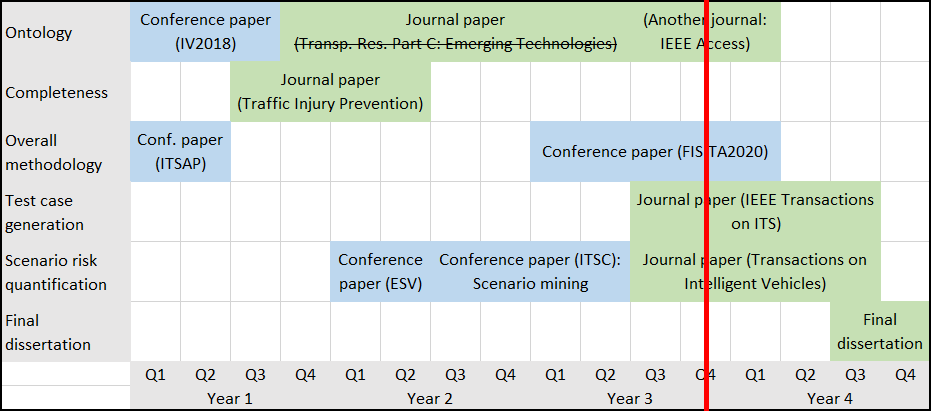
\includegraphics[width=\linewidth]{planning.png}
%	\caption{Proposed planning at the time of this report. The red line indicated the time when writing this report.}
%	\label{fig:planning}
%\end{figure}

\begin{itemize}
	\item I would like to work out the contents of the article on the scenario risk quantification. I am thinking of doing that first in a PowerPoint presentation, because that allows for easier discussion internally at TNO. Once we agree on the contents, I hope to quickly start writing.
	\item Continue to work on the test case generation.
\end{itemize}


\printbibliography

%\clearpage
%\includepdf[pages=-,pagecommand={},width=\paperwidth]{../../""/.pdf}

\end{document}